% This work is made available under the terms of the
% Creative Commons Attribution-ShareAlike 4.0 license,
% http://creativecommons.org/licenses/by-sa/4.0/.

\documentclass[a4paper]{book}

\usepackage{wrapfig}
\usepackage{graphicx}
\usepackage{hyperref}
\usepackage{multirow}
\usepackage{scalefnt}
\usepackage{tikz}

% watermark -- for draft stage
%\usepackage[firstpage]{draftwatermark}
%\SetWatermarkLightness{0.9}
%\SetWatermarkScale{5}

% Copyright (c) 2009 by the University of Waikato, Hamilton, NZ. 
% This work is made available under the terms of the 
% Creative Commons Attribution-ShareAlike 4.0 license,
% http://creativecommons.org/licenses/by-sa/4.0/.
%
% Version: $Revision: 13214 $

\newenvironment{tight_itemize}{
\begin{itemize}
  \setlength{\itemsep}{1pt}
  \setlength{\parskip}{0pt}
  \setlength{\parsep}{0pt}}{\end{itemize}
}

\newenvironment{tight_enumerate}{
\begin{enumerate}
  \setlength{\itemsep}{1pt}
  \setlength{\parskip}{0pt}
  \setlength{\parsep}{0pt}}{\end{enumerate}
}

% if you just need a simple heading
% Usage:
%   \heading{the text of the heading}
\newcommand{\heading}[1]{
  \vspace{0.3cm} \noindent \textbf{#1} \newline
}

\newcommand{\icon}[1]{\tikz[baseline=-3pt]\node[inner sep=0pt,outer sep=0pt]{\includegraphics[height=1.1em]{#1}};}


\title{
  \textbf{ADAMS} \\
  {\Large \textbf{A}dvanced \textbf{D}ata mining \textbf{A}nd \textbf{M}achine
  learning \textbf{S}ystem} \\
  {\Large Module: adams-weka-lts} \\
  \vspace{1cm}
  \includegraphics[width=2cm]{images/weka-lts-module.png} \\
}
\author{
  Peter Reutemann
}

\setcounter{secnumdepth}{3}
\setcounter{tocdepth}{3}

\begin{document}

\begin{titlepage}
\maketitle

\thispagestyle{empty}
\center
\begin{table}[b]
	\begin{tabular}{c l l}
		\parbox[c][2cm]{2cm}{\copyright 2009-2025} &
		\parbox[c][2cm]{5cm}{
\includegraphics[width=5cm]{images/coat_of_arms.pdf}} \\
	\end{tabular}
	
\includegraphics[width=12cm]{images/cc.png} \\
\end{table}

\end{titlepage}

\tableofcontents
\listoffigures
%\listoftables

%%%%%%%%%%%%%%%%%%%%%%%%%%%%%%%%%%%
\chapter{Introduction}
The \textit{adams-weka} module offers most of the functionality found in WEKA
\cite{weka}: pre-processing, classification and regression, clustering,
attribute selection, data visualization and visualization of results/models.
But it does not stop there: the module also contains other features for
optimization, experiment generation that are not available from WEKA, be it
Explorer or KnowledgeFlow. It is assumed that you are familiar with
WEKA\footnote{If you haven't used WEKA before, check out the Data Mining book
\cite{wekabook}, which gives you a good introduction to machine learning, data
mining and WEKA.} and machine learning in general, as common terms are not
explained again.

If you have used WEKA's KnowledgeFlow before, then you will have to forget
(mostly) everything that you know about setting up workflows. ADAMS does things
quite differently in comparison to the WEKA. Additionally, ADAMS offers a range
of general purpose actors that allow you to go further.

The manual is split into several sections, with: \textit{classification and regression}
and \textit{clustering} comprising the most important sections.

% This work is made available under the terms of the
% Creative Commons Attribution-ShareAlike 4.0 license,
% http://creativecommons.org/licenses/by-sa/4.0/.

\chapter{Flow}
The \textit{adams-weka} module has a comprehensive set of actors and conversions
that allow you to build powerful flows using WEKA's functionality. The following
sections give a quick overview of available functionality. If you are interested
in flow examples, check out chapters \ref{classification_and_regression} and
\ref{clustering}.

\section{Conversions}
This module offers additional schemes for the \textit{Convert} transformer:
\begin{tight_itemize}
	\item \textit{AdamsInstanceToWekaInstance} -- converts an ADAMS instance
	into a WEKA one.
	\item \textit{MatchWekaInstanceAgainstFileHeader} -- uses a dataset header
	stored in a file to convert the string attributes of the instance passing 
	through into nominal ones (and vice versa).
	\item \textit{MapToWekaInstance} -- turns a java.util.Map object into
	an Instance object using a dataset in storage as template.
	\item \textit{MatchWekaInstanceAgainstStorageHeader} -- uses a dataset
	header obtained from storage to convert the string attributes of the 
	instance passing through into nominal ones (and vice versa).
	\item \textit{ReportToWekaInstance} -- turns a \textit{Report} object
	into a WEKA instance.
	\item \textit{SpreadSheetToWekaInstances} -- turns a spreadsheet object
	into a WEKA dataset.
	\item \textit{WekaCapabilitiesToInstances} -- generates a dataset with
	random data that adheres to the capabilities retrieved from a
	\texttt{CapabilitiesHandler}.
	\item \textit{WekaDrawableString} -- exports the graph from a decision
	tree or bayesian network in 'dot' notation.
	\item \textit{WekaEvaluationToCostCurve} -- turns an Evaluation into
	cost curve data.
	\item \textit{WekaEvaluationToMaringCurve} -- turns an Evaluation into
	margin curve data.
	\item \textit{WekaEvaluationToThresholdCurve} -- turns an Evaluation into
	threshold curve data (eg ROC).
	\item \textit{WekaCapabilitiesToSpreadSheet} -- generates a spreadsheet
	with the  capabilities retrieved from a \texttt{CapabilitiesHandler}.
	\item \textit{WekaCommandToCode} -- turns a WEKA command-line into
	code snippets.
	\item \textit{WekaInstanceToMap} -- turns an Instance object into a
	java.util.Map object.
	\item \textit{WekaInstancesToSpreadSheet} -- turns a WEKA dataset into
	a spreadsheet object.
	\item \textit{WekaInstanceToAdamsInstance} -- turns a WEKA instance into
	an ADAMS one.
	\item \textit{WekaPredictionContainerToSpreadSheet} -- generates a 
	spreadsheet object from a prediction container (useful for display).
\end{tight_itemize}

\section{Conditions}
The following boolean conditions, e.g., used in the \textit{IfThenElse} or
\textit{Switch} control actors, are available:
\begin{tight_itemize}
	\item \textit{AdamsInstanceCapabilities} -- checks an ADAMS intance against
	the specified capabilities that it must satisfy.
	\item \textit{WekaCapabilities} -- checks a WEKA instance against the
	specified capabilities.
	\item \textit{WekaClassification} (used in conjunction with 
	\textit{Switch}) -- uses the returned classification index to determine 
	which branch of the switch statement should be used; for all other control 
	actors, the condition evaluates to ``true'' if an index is returnedl; 
	condition works only with nominal classes.
\end{tight_itemize}

\section{Actors}
The following sources are available:
\begin{tight_itemize}
	\item \textit{WekaAssociatorSetup} -- outputs a single associator setup.
	\item \textit{WekaClassifierGenerator} -- generates parameter sweeps for
	\item \textit{WekaClassifierSetup} -- outputs a single classifier setup.
	\item \textit{WekaClustererGenerator} -- generates parameter sweeps for
	\item \textit{WekaClustererSetup} -- outputs a single clusterer setup.
	\item \textit{WekaDatabaseReader} -- reads data from a database into
	WEKA's internal format.
	\item \textit{WekaDataGenerator} -- generates artificial data using WEKA's
	data generators.
	\item \textit{WekaFilterGenerator} -- generates parameter sweeps for
	filters.
	\item \textit{WekaNewExperiment} -- creates a new ADAMS experiment setup.
	\item \textit{WekaNewInstances} -- for generating empty datasets.
	\item \textit{WekaSelectDataset} -- for selecting datasets interactively.
	\item \textit{WekaSelectObjects} -- for selecting Weka objects, like
	classifiers.
\end{tight_itemize}
These transformers:
\begin{tight_itemize}
	\item \textit{WekaAccumulatedError} -- extracts all the errors
	collected during an evaluation, sorted according to magnitude and
	creates plot output, for comparing classifier performances (most useful
	for numeric classes).
	\item \textit{WekaAggregatedEvaluations} -- aggregates incoming
	Evaluation objects and forwards the current, aggregate state. 
	\item \textit{WekaAttributeIterator} -- iterates through the names of a
	dataset and outputs them.
	\item \textit{WekaAttributeSelection} -- for performing attribute selection.
	\item \textit{WekaAttributeSelectionSummary} -- generates a summary of the
	incoming attribute selection data.
	\item \textit{WekaBootstrapping} -- performs bootstrapping\footnote{\url{https://en.wikipedia.org/wiki/Bootstrapping\_\%28statistics\%29}{}}
	on the incoming evaluation data and outputs a spreadsheet.
	\item \textit{WekaChooseAttributes} -- allows the user to interactively
	select attributes to keep in a dataset.
	\item \textit{WekaClassifierInfo} -- outputs basic information about
	a classifier.
	\item \textit{WekaClassifierOptimizer} -- applies a classifier optimizer
	(e.g., GridSearch or MultiSearch) to a dataset and then forwards the best
	(untrained) setup.
	\item \textit{WekaClassifierRanker} -- evaluates an array of classifier
	setups on a dataset and outputs the top X performing setups.
	\item \textit{WekaClassifierSetupProcessor} -- processes the incoming array
	of classifiers and outputs a new one.
	\item \textit{WekaClassifying} -- uses a serialized (or callable) model to
	make predictions on incoming data.
	\item \textit{WekaClassSelector} -- sets the class attribute in a dataset.
	\item \textit{WekaClusterAssignments} -- outputs the cluster assignments
	from a cluster evaluation.
	\item \textit{WekaClustererInfo} -- outputs basic info about a clusterer.
	\item \textit{WekaClusterEvaluationSummary} -- generates a summary string
	from a cluster evaluation object.
	\item \textit{WekaClustering} -- applies a serialized (or callable) model
	to incoming data.
	\item \textit{WekaCrossValidationClustererEvaluator} -- performs cross-validation
	on an incoming dataset using the referenced clusterer setup.
	\item \textit{WekaCrossValidationEvaluator} -- performs cross-validation
	on an incoming dataset using the referenced classifier setup.
	\item \textit{WekaCrossValidationSplit} -- generates train/test set splits
	like cross-validation would generate.
	\item \textit{WekaDatasetsMerge} -- like \textit{WekaInstancesMerge},
	allows the merging of several datasets (side-by-side), but uses a class
	hierarchy of merge algorithms.
	\item \textit{WekaEvaluationInfo} -- outputs basic info about a Weka
	Evaluation object.
	\item \textit{WekaEvaluationPostProcessor} -- allows post-processing
	of Evaluation objects, e.g., extraction sub-ranges.
	\item \textit{WekaEvaluationSummary} -- generates a summary for an
	Evaluation.
	\item \textit{WekaEvaluationValuePicker} -- retrieves a single statistic
	from an Evaluation.
	\item \textit{WekaEvaluationValues} -- generates a spreadsheet with the
	selected statistics from an Evaluation.
	\item \textit{WekaExperiment} -- executes a WEKA experiment, like in the 
	Experimenter.
	\item \textit{WekaExperimentEvaluation} -- evaluates a WEKA experiment,
	generating text output of various sorts.
	\item \textit{WekaExperimentExecution} -- executes an incoming ADAMS
	experiment.
	\item \textit{WekaExperimentFileReader} -- reads an experiment from disk.
	\item \textit{WekaExtractArray} -- extracts a row or column from a WEKA
	dataset (using the internal format).
	\item \textit{WekaExtractPLSMatrix} -- extracts PLS matrices from in
	incoming PLS classifier (or scheme that gives access to internal PLS matrices).
	\item \textit{WekaFileReader} -- reads any dataset that WEKA can handle,
	either outputs the header, the complete dataset or row-by-row.
	\item \textit{WekaFilter} -- applies a WEKA filter to the data.
	\item \textit{WekaGenericPLSMatrixAccess} -- extracts PLS matrices from in
	incoming PLS classifier (or scheme that gives access to internal PLS matrices).
	\item \textit{WekaGeneticAlgorithm} -- applies the specified genetic
	algorithm to the incoming dataset, e.g., for parameter optimization.
	\item \textit{WekaGeneticAlgorithmInitializer} -- generates a container
	with a genetic algorithm and training data to prime a WekaGeneticAlgorithm
	transformer with.
	\item \textit{WekaGetCapabilities} -- retrieves the capabilities of a
	\texttt{CapabilitiesHandler} (e.g., Filter or Classifier).
	\item \textit{WekaGetInstanceValue} -- retrieves an attribute's value from
	a dataset row.
	\item \textit{WekaGetInstancesValue} -- retrieves an attribute's value from
	a dataset.
	\item \textit{WekaInstanceBuffer} -- buffers either incoming instance 
	objects and outputs datasets or outputs instance objects when getting
	datasets.
	\item \textit{WekaInstanceDumper} -- for dumping dataset rows into files,
	one row at a time (ARFF or CSV).
	\item \textit{WekaInstanceEvaluator} -- adds an attribute with the value
	returned by an instance evaluator.
	\item \textit{WekaInstanceFileReader} -- outputs ADAMS instance objects.
	\item \textit{WekaInstancesAppend} -- creates one large dataset from 
	multiple ones, by appending them one after the other.
	\item \textit{WekaInstancesHistogramRanges} -- outputs the ranges generated by the
	ArrayHistogram statistic.
	\item \textit{WekaInstancesInfo} -- outputs information on a dataset.
	\item \textit{WekaInstancesMerge} -- allows the merging of several datasets 
	(side-by-side).
	\item \textit{WekaInstancesStatistic} -- computes statistics on rows
	or columns of an Instances object.
	\item \textit{WekaInstanceStreamPlotGenerator} -- generates plot containers
	from a range of attributes of instance objects passing through (i.e., you 
	can plot several attributes in one go).
	\item \textit{WekaModelReader} -- reads a serialized model.
	\item \textit{WekaMultiLabelSplitter} -- splits a datasets with multiple
	class attributes (``multi-label'') into ones with only a single class 
	attribute.
	\item \textit{WekaNearestNeighborSearch} -- determines the neighborhood
	for incoming Instance objects.
	\item \textit{WekaNewInstance} -- creates an instance object with only
	missing values using a dataset as template.
	\item \textit{WekaPredictionsToInstances} -- turns WEKA predictions into
	a WEKA dataset (actual, predicted, etc).
	\item \textit{WekaPredictionsToSpreadSheet} -- turns WEKA predictions into
	a spreadsheet (actual, predicted, etc).
	\item \textit{WekaPrincipalComponents} -- outputs loadings and transformed
	data obtained from principal components analysis.
	\item \textit{WekaRandomSplit} -- generates a random split of a dataset.
	\item \textit{WekaRegexToRange} -- generates a range string using a regular
	expression applied to the names of a dataset.
	\item \textit{WekaRenameRelation} -- renames a dataset.
	\item \textit{WekaReorderAttributesToReference} -- reorders the attributes
	in incoming Instance/Instances based on an order defined in a reference
	dataset (callable actor or file).
	\item \textit{WekaRepeatedCrossValidationEvaluator} -- performs repeated
	cross-validation on an incoming dataset using the referenced classifier setup.
	\item \textit{WekaRepeatedCrossValidationOutput} -- generates output
	from the repeated cross-validation data.
	\item \textit{WekaSetInstanceValue} -- sets a specific attribute value in
	an instance object.
	\item \textit{WekaSetInstancesValue} -- sets a specific attribute value in
	a dataset object.
	\item \textit{WekaSpreadSheetToPredictions} -- turns a spreadsheet back
	into a fake Evaluation object. Allows processing of actual/predicted data
	from other applications.
	\item \textit{WekaStoreInstance} -- appends the passing through instance
	\item \textit{WekaStreamEvaluator} -- performs prequential evaluation
	of an incremental classifier on a data stream.
	\item \textit{WekaStreamFilter} -- works the same as
	\textit{WekaFilter} but only allows stream filters to be selected.
	\item \textit{WekaSubsets} -- splits dataset into subsets using the unique
	values of an attribute to identify subsets.
	\item \textit{WekaTestSetClustererEvaluator} -- evaluates a trained
	clusterer on a dataset obtained from a callable actor.
	\item \textit{WekaTestSetEvaluator} -- evaluates a trained classifier on
	a dataset obtained from a callable actor.
	\item \textit{WekaTextDiectoryReader} -- reads in a directory with the 
	documents in the sub-directories representing different classes.
	\item \textit{WekaTrainAssociator} -- used for building an associator
	on a dataset.
	\item \textit{WekaTrainClassifier} -- used for generating a trained
	model using a dataset.
	\item \textit{WekaTrainClusterer} -- trains a cluster algorithm setup
	on a dataset.
	\item \textit{WekaTrainTestSetClustererEvaluator} -- evaluates a referenced
	clusterer using the incoming train/test split.
	\item \textit{WekaTrainTestSetEvaluator} -- evaluates a referenced classifier
	using the incoming train/test split.
\end{tight_itemize}
And these sinks:
\begin{tight_itemize}
	\item \textit{WekaAttributeSummary} -- displays the summary of one or more attributes.
	\item \textit{WekaClassifierErrors} -- displays the errors of a classifier.
	\item \textit{WekaCostBenefitAnalysis} -- displays a cost-benefit analysis dialog.
	\item \textit{WekaCostCurve} -- generates a cost curve.
	\item \textit{WekaDatabaseWriter} -- writes a dataset to a database.
	\item \textit{WekaExperimentFileWriter} -- writes an ADAMS experiment to disk.
	\item \textit{WekaExperimentGenerator} -- generates a WEKA experiment by
	adding the incoming classifier setups and writing it to disk.
	\item \textit{WekaFileWriter} -- writes a dataset to any file format that
	WEKA can handle.
	\item \textit{WekaGraphVisualizer} -- displays a Bayesian network (from XML or BIF).
	\item \textit{WekaInstancesDisplay} -- displays datasets in table format.
	\item \textit{WekaInstancesPlot} -- plots one attribute vs another.
	\item \textit{WekaInstanceViewer} -- visualizes incoming WEKA or ADAMS
	instance objects the same way as the \textit{Instance Explorer} tool does.
	\item \textit{WekaMarginCurve} -- displays a margin curve.
	\item \textit{WekaModelWriter} -- writes a model container or
	classifier/clusterer to disk.
	\item \textit{WekaThresholdCurve} -- displays threshold curves like, 
	receiver-operator curve (ROC) or precision/recall.
	\item \textit{WekaTreeVisualizer} -- displays a tree in 'dot' notation.
\end{tight_itemize}

\section{Templates}
Here are some templates that make the flow development for WEKA easier:
\begin{tight_itemize}
	\item \textit{InstanceDumperVariable} -- generates a variable for the 
	\textit{WekaInstanceDumper} actor which contains an ARFF/CSV filename 
	prefix aligned with the flow's filename, i.e., the ARFF/CSV file will 
	always get placed in the same location as the flow.
\end{tight_itemize}


\include{classification_and_regression}

\include{clustering}

% This work is made available under the terms of the
% Creative Commons Attribution-ShareAlike 4.0 license,
% http://creativecommons.org/licenses/by-sa/4.0/.

\chapter{Attribute selection}
\label{attribute_selection}
ADAMS also offers WEKA's functionality for attribute selection and ranking.
The following transformers are available:
\begin{tight_itemize}
	\item \textit{WekaAttributeSelection} -- performs the attribute 
	selection/ranking.
	\item \textit{WekaAttributeSelectionSummary} -- generates a summary from
	a attribute selection step.
\end{tight_itemize}

In Figure \ref{attribute-selection_flow} you can see a flow\footnote{adams-weka-attribute\_selection-subset.flow} 
that uses \textit{CfsSubsetEval} as the attribute set evaluator and \textit{BestFirst}
as the search method. The generated output, summary and reduced dataset,
are displayed in Figures \ref{attribute-selection_output1} and 
\ref{attribute-selection_output2}.

\begin{figure}[htb]
  \centering
  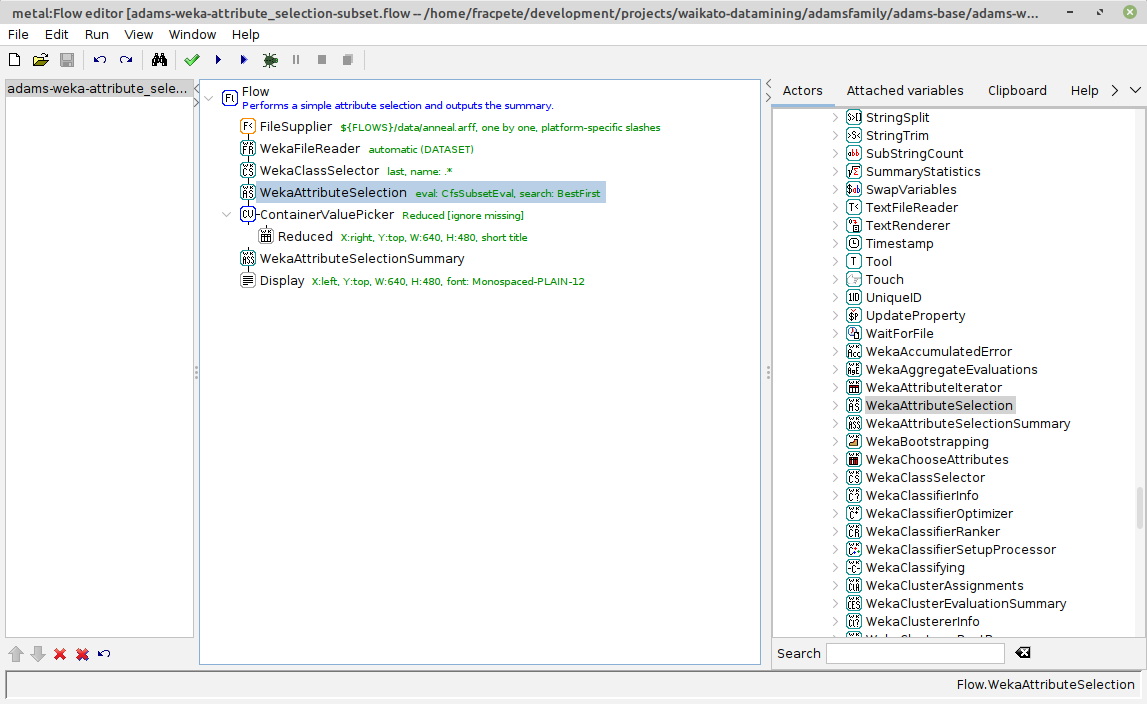
\includegraphics[width=6.0cm]{images/attribute-selection_flow.png}
  \caption{Flow for performing attribute selection (reduction).}
  \label{attribute-selection_flow}
\end{figure}

\begin{figure}[ht]
  \begin{minipage}[t]{0.5\linewidth}
    \centering
    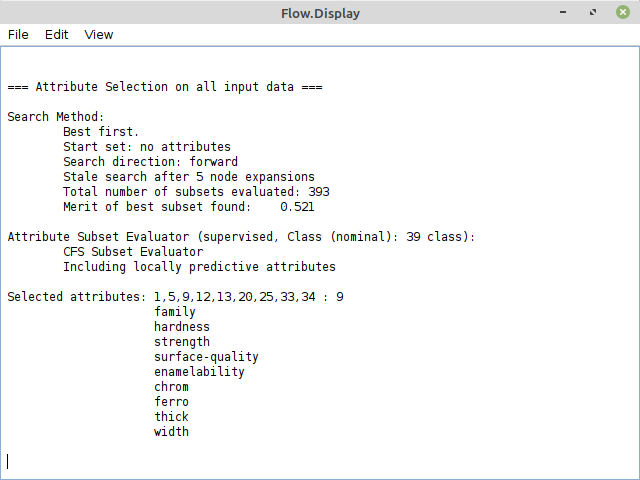
\includegraphics[width=6.0cm]{images/attribute-selection_output1.png}
    \caption{Summary of the reduction.}
    \label{attribute-selection_output1}
  \end{minipage}
  \hspace{0.5cm}
  \begin{minipage}[t]{0.5\linewidth}
    \centering
    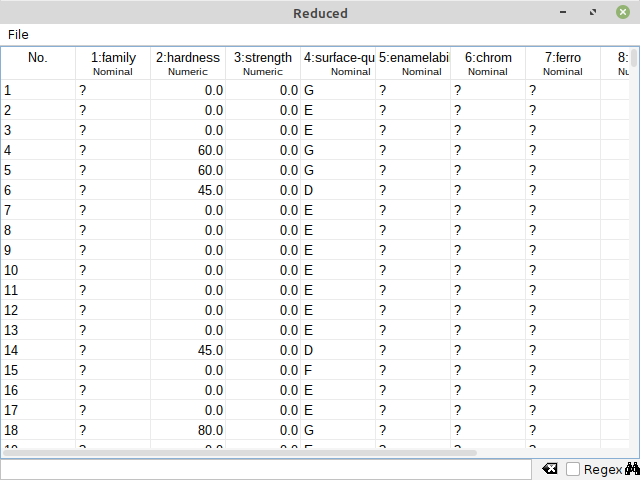
\includegraphics[width=5.5cm]{images/attribute-selection_output2.png}
    \caption{The reduced dataset.}
    \label{attribute-selection_output2}
  \end{minipage}
\end{figure}

The \textit{WekaAttributeSelection} transformer outputs a container which can 
contain the following elements:
\begin{tight_itemize}
	\item \textit{Train} -- the training set.
	\item \textit{Reduced} -- the reduced dataset.
	\item \textit{Transformed} -- the transformed dataset, in case of evaluators that 
	implement \textit{AttributeTransformer}, like principal components.
	\item \textit{Evaluation} -- the generated attribute selection evaluation.
	\item \textit{Statistics} -- a spreadsheet with statistics, containing
	information whether an attribute was selected (0 or 1) or for ranking results
	the rank of the attribute.
	\item \textit{Seed} -- the seed value in case of cross-validation.
	\item \textit{Folds} -- the number of folds used in case of cross-validation.
\end{tight_itemize}


% This work is made available under the terms of the
% Creative Commons Attribution-ShareAlike 4.0 license,
% http://creativecommons.org/licenses/by-sa/4.0/.

\chapter{Associations}
\label{associations}

Associators in WEKA are very limited in terms what you can do with them: you
can build an associator and output its rules, it the algorithm supports it.
The flow\footnote{adams-weka-associator.flow} in Figure \ref{associator}
shows how to train an associator using the \textit{WekaTrainAssociator}
transformer, which uses the Apriori setup obtained from the \textit{WekaAssociatorSetup}
source, and outputs the Apriori model and the rules that Apriori generated.

\begin{figure}[htb]
  \centering
  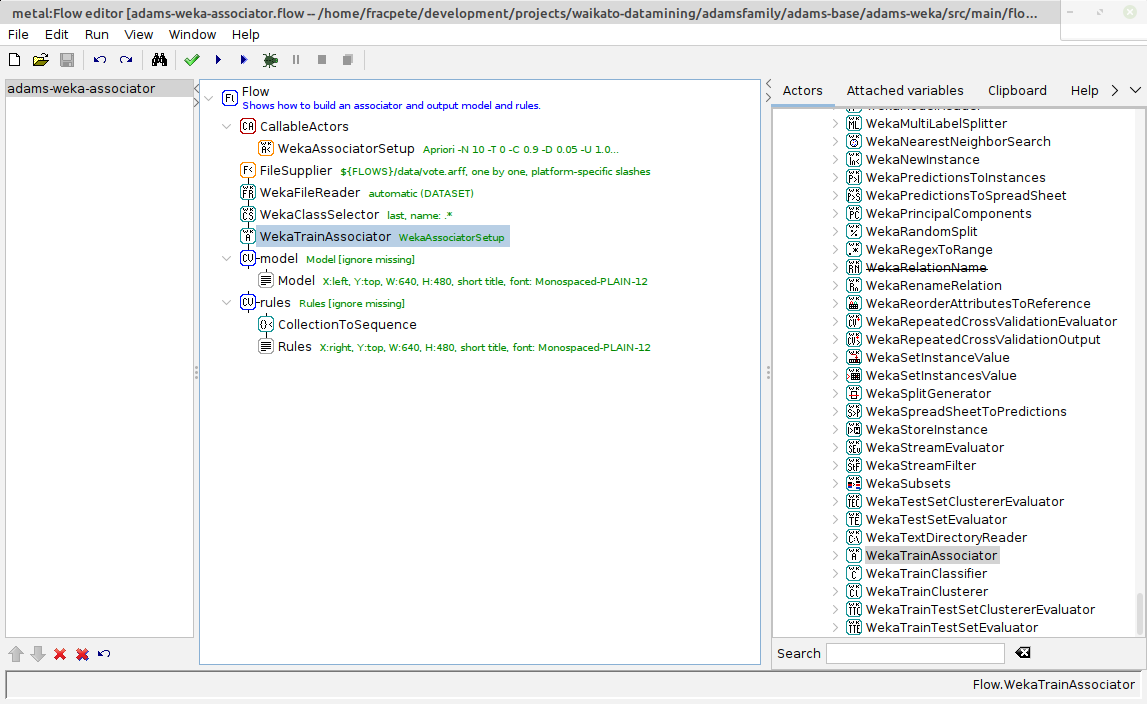
\includegraphics[width=12.0cm]{images/associator.png}
  \caption{Flow for building an associator and outputting model and rules.}
  \label{associator}
\end{figure}


\include{visualization}

% This work is made available under the terms of the
% Creative Commons Attribution-ShareAlike 4.0 license,
% http://creativecommons.org/licenses/by-sa/4.0/.

\chapter{Machine learning}

\section{Dark Lord}
The \textit{Dark Lord} wizard allows you to set up and monitor a genetic
algorithm that determines the best set of attributes, based on the classifier
and metric you choose to optimize on. The output directory that you define
(see Figure \ref{darklord_setup}), is used to store all the \textit{reduced/optimized}
datasets that improved the metric and the classifier configurations. The following screenshots were obtained for
the \textit{triazines} regression dataset\footnote{\url{}{https://sourceforge.net/projects/weka/files/datasets/regression-datasets/regression-datasets.jar/download}}
using 1,000 iterations, notifications sent whenever a change occurs (``notificationInterval'' is 0)
and LinearRegression as classifier (with all attribute selection turned off).
The optimization can be paused, resumed or stopped with the buttons at the
bottom right of the view panel (see Figure \ref{darklord_run}).

\begin{figure}[htb]
  \centering
  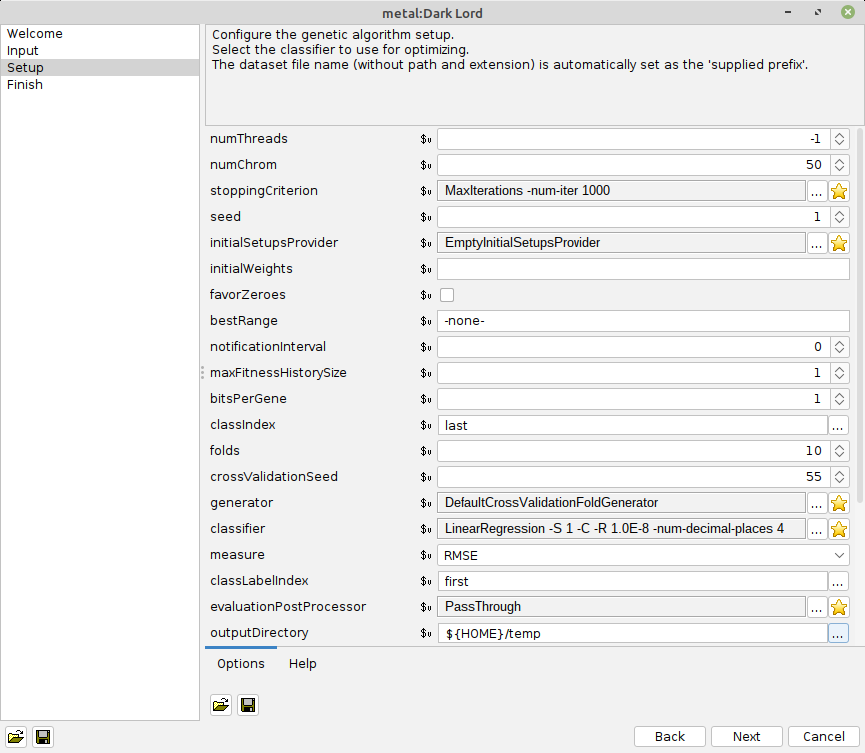
\includegraphics[width=12.0cm]{images/darklord_setup.png}
  \caption{Dark Lord setup.}
  \label{darklord_setup}
\end{figure}

\begin{figure}[htb]
  \centering
  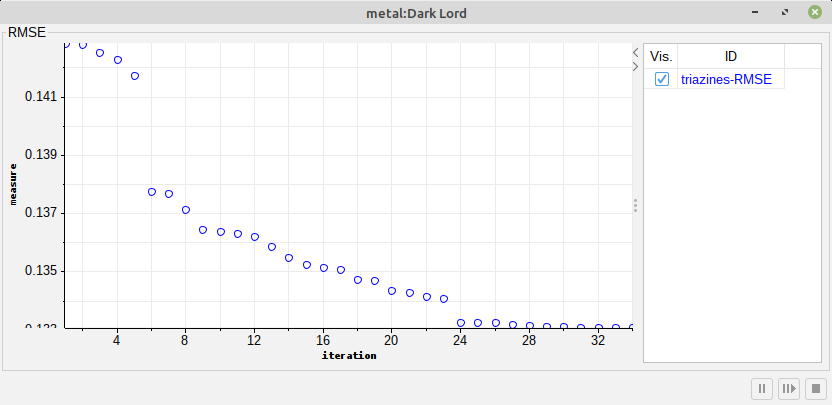
\includegraphics[width=12.0cm]{images/darklord_run.png}
  \caption{Dark Lord run.}
  \label{darklord_run}
\end{figure}

\clearpage
\section{Hermione}
The \textit{Hermione} wizard allows you to set up and monitor a genetic
algorithm that determines the best parameter settings, based on the classifier
and metric you choose to optimize on. The output directory that you define
(see Figure \ref{hermione_setup}), is used to store all the setups/datasets
that improved the metric. The optimization can be paused, resumed or
stopped with the buttons at the bottom right of the view panel (see Figure
\ref{hermione_run}). The screenshots were generated from optimizing
the GPD classifier's gamma/noise and the PLS filter's components (both wrapped
in a FilteredClassifier) on the \textit{triazines} regression
dataset\footnote{\url{}{https://sourceforge.net/projects/weka/files/datasets/regression-datasets/regression-datasets.jar/download}}.

\begin{figure}[htb]
  \centering
  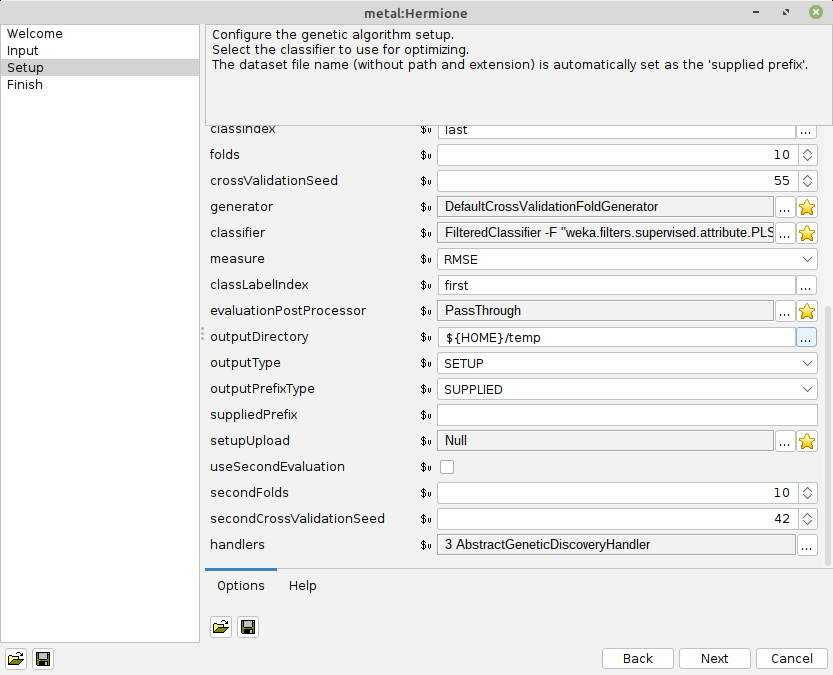
\includegraphics[width=12.0cm]{images/hermione_setup.png}
  \caption{Hermione setup.}
  \label{hermione_setup}
\end{figure}

\begin{figure}[htb]
  \centering
  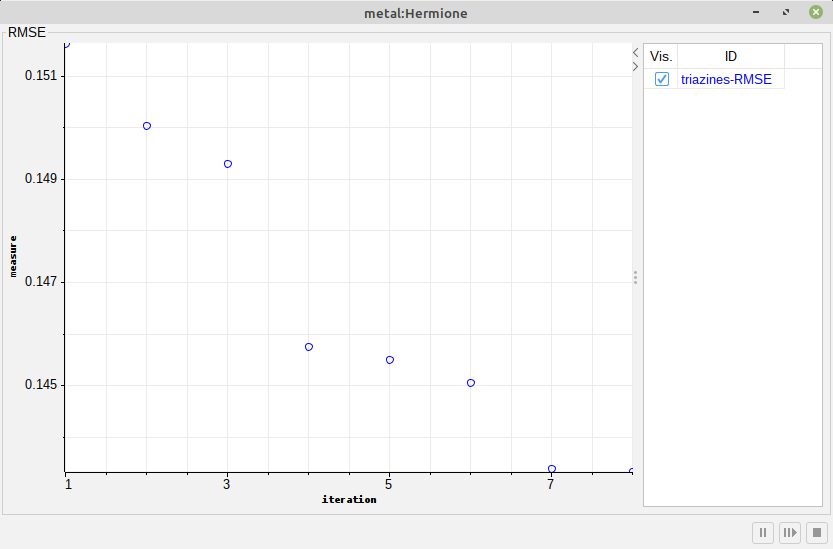
\includegraphics[width=10.0cm]{images/hermione_run.png}
  \caption{Hermione run.}
  \label{hermione_run}
\end{figure}

\clearpage
\section{WEKA Experimenter}
The classic interface of the \textit{WEKA Experimenter} is available in ADAMS as well.

\begin{figure}[htb]
  \centering
  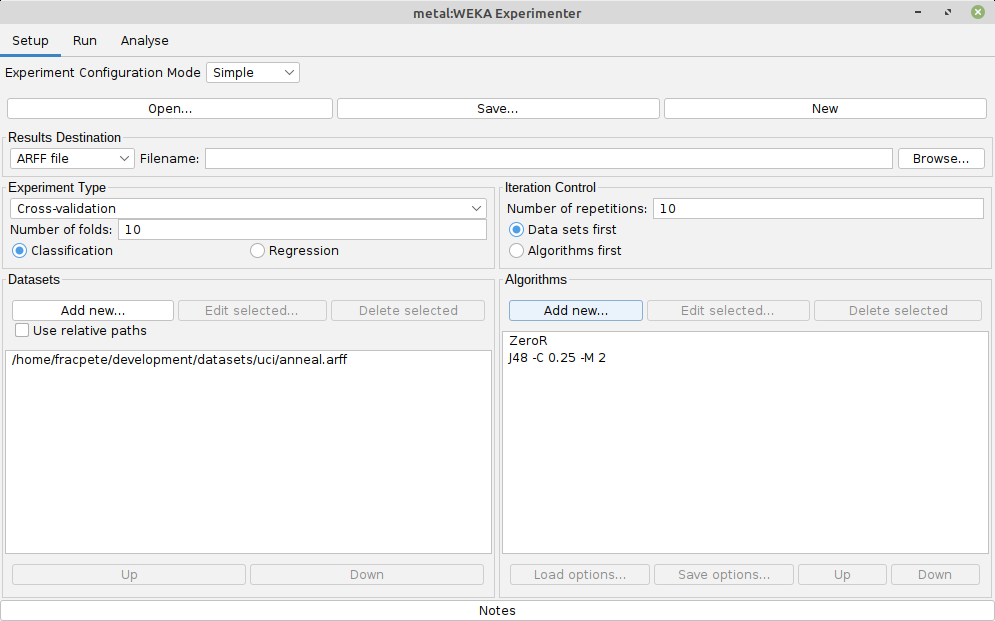
\includegraphics[width=12.0cm]{images/experimenter.png}
  \caption{Experimenter interface.}
  \label{experimenter}
\end{figure}

\clearpage
\section{WEKA Explorer}
The classic interface of the \textit{WEKA Explorer} is available in ADAMS as well.

\begin{figure}[htb]
  \centering
  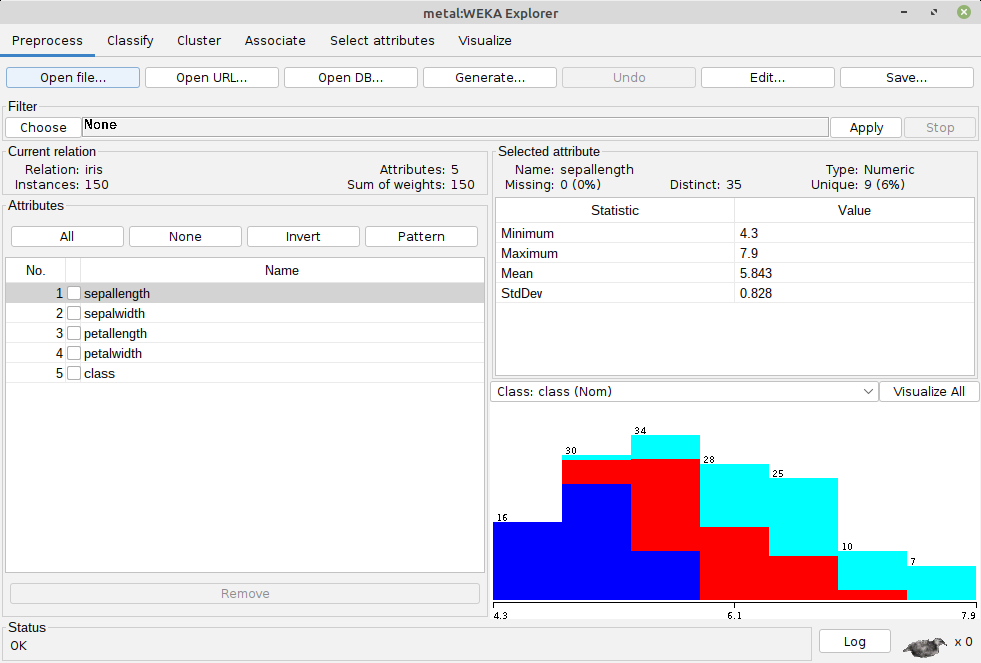
\includegraphics[width=12.0cm]{images/explorer.png}
  \caption{Explorer interface.}
  \label{explorer}
\end{figure}

\clearpage
\section{WEKA Investigator}
The \textit{WEKA Investigator} (see Figure \ref{wekainvestigator}) is aimed
to be a replacement of the WEKA Explorer. The idea is to have a more versatile
and efficient user interface: manage multiple sessions, each session can manage
multiple datasets (e.g., train and test set), making use of tabs instead of windows
(but output tabs can still be detached for comparison), configuration of
outputs to generate each time an evaluation is run (statistics, model,
classifier errors, etc).

\begin{figure}[htb]
  \centering
  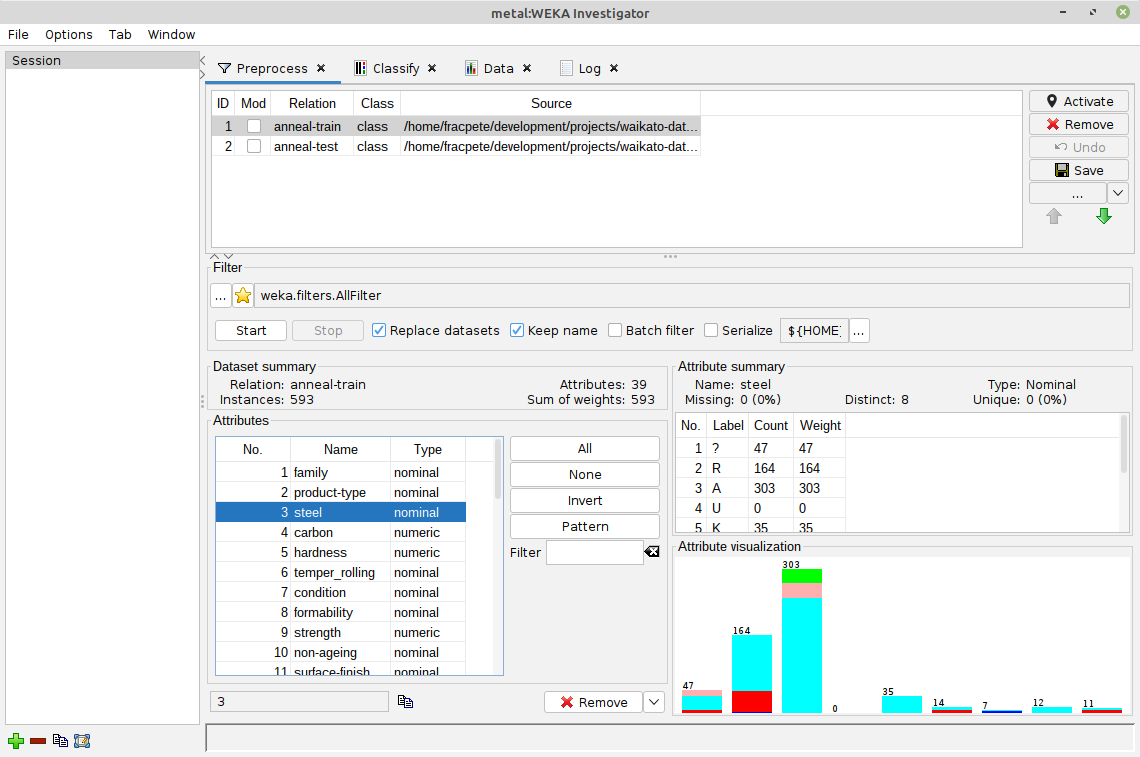
\includegraphics[width=12.0cm]{images/wekainvestigator.png}
  \caption{Weka Investigator.}
  \label{wekainvestigator}
\end{figure}

\clearpage
\section{WEKA Multi-Experimenter}
The \textit{Multi-Experimenter} interface allows multiple sessions within the same window,
as well as being able to run ADAMS or WEKA experiments. The statistical evaluation is
using WEKA's underlying API in both cases.

\begin{figure}[htb]
  \centering
  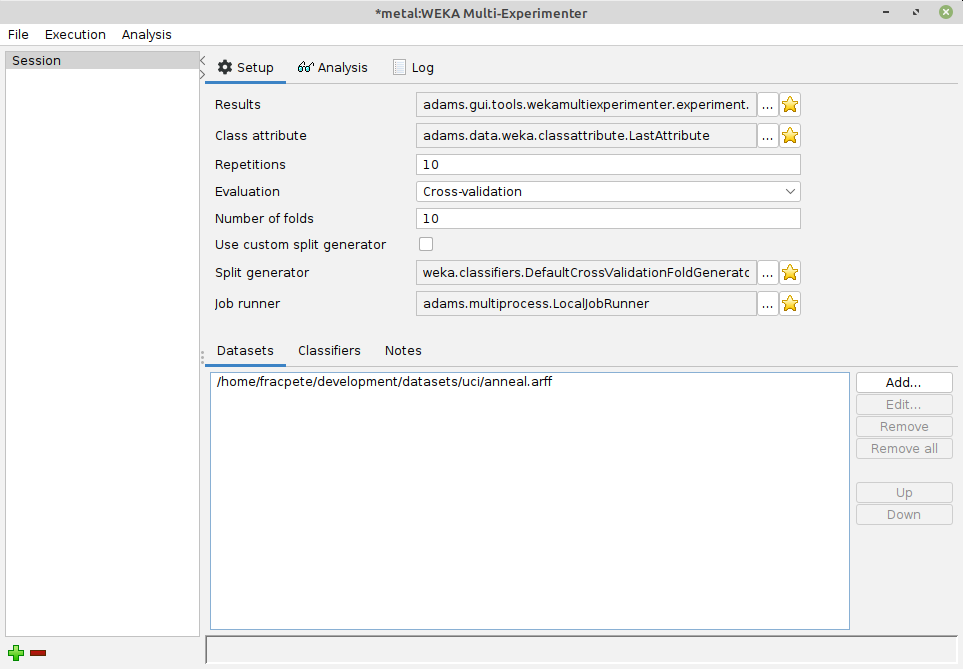
\includegraphics[width=12.0cm]{images/multi-experimenter.png}
  \caption{Multi-Experimenter.}
  \label{multi-experimenter}
\end{figure}

\clearpage
\section{WEKA Multi-Explorer}
ADAMS contains an extended version of the WEKA Explorer. The interface uses
menus instead of buttons to declutter the pre-process tab. Also, it keeps track
of the datasets that the user loads, to make re-loading recent files easier.
This saves a lot of time when working with the same files on a frequent basis.
Furthermore, the user can have an arbitrary number of Explorer sessions in the
same window, distinguished by names. Figure \ref{explorerext} shows the new
interface with the drop-down menu in action.

\begin{figure}[htb]
  \centering
  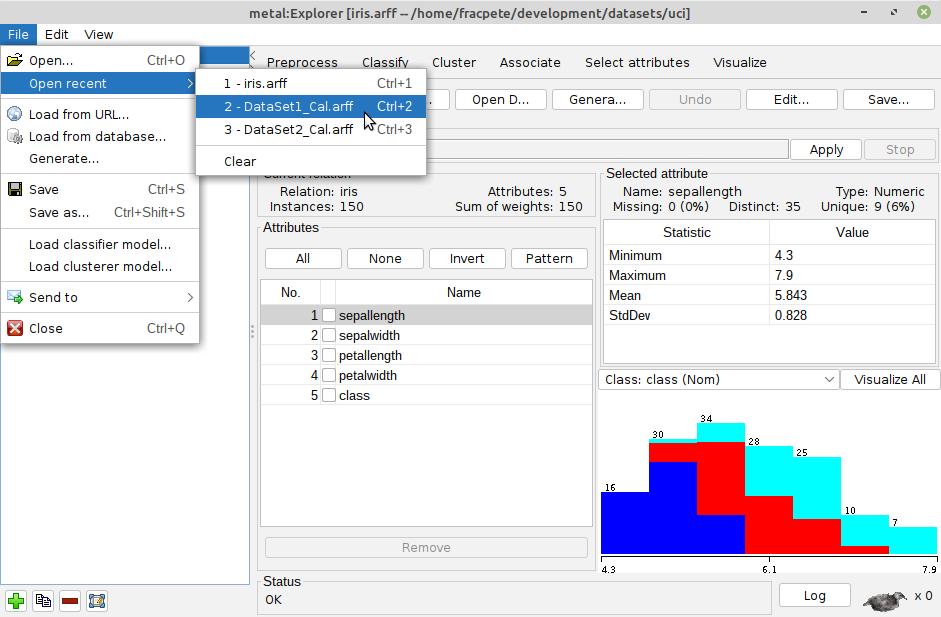
\includegraphics[width=12.0cm]{images/explorerext.png}
  \caption{Explorer interface with menus.}
  \label{explorerext}
\end{figure}

One very useful feature is the notion of \textit{workspaces} in this interface.
You can save the current setup (current dataset, classifiers, clusterers,
evaluation set up, results, etc.) to a file and restore all of it in one go
again. Unfortunately, not all data can be stored, such as the log, the undo
history and the built models or visualizations associated with a results.
See Figure \ref{explorerext-workspaces} for the button (highlighted in red)
that allows you to load/save workspaces.

\begin{figure}[htb]
  \centering
  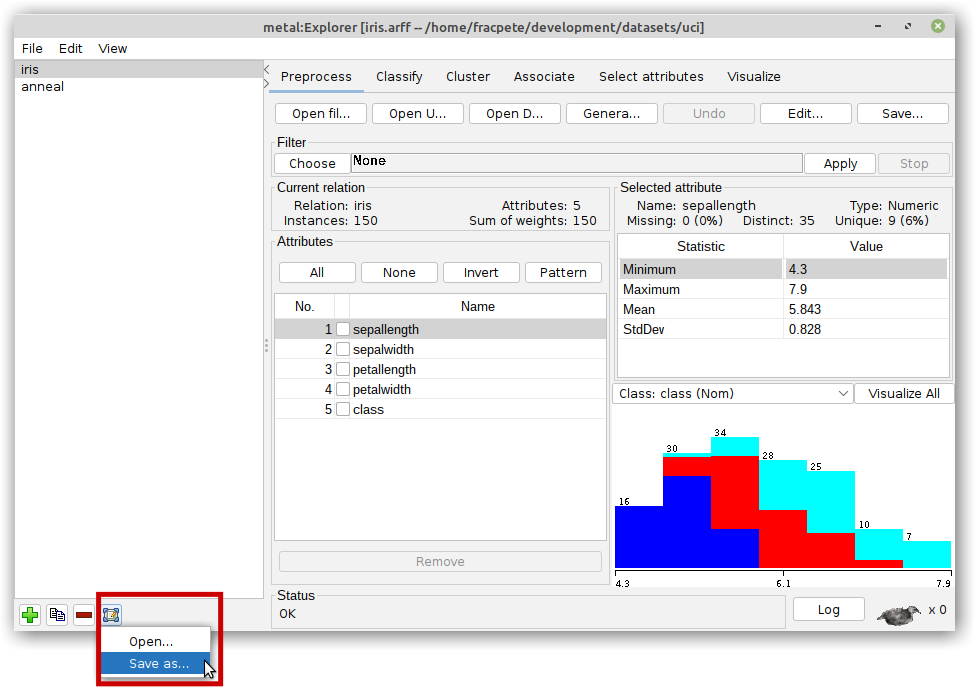
\includegraphics[width=12.0cm]{images/explorerext-workspaces.png}
  \caption{Saving/restoring of workspaces.}
  \label{explorerext-workspaces}
\end{figure}

\clearpage
\section{WEKA SimpleCLI}
Weka's basic command-line interface, \textit{SimpleCLI}, is also
available. A screenshot is shown in Figure \ref{simplecli}.

\begin{figure}[htb]
  \centering
  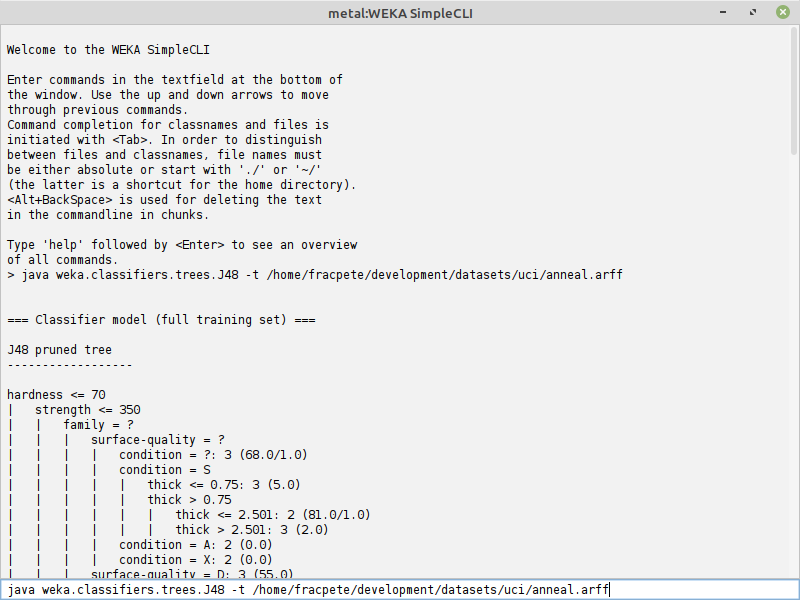
\includegraphics[width=12.0cm]{images/simplecli.png}
  \caption{The SimpleCLI interface.}
  \label{simplecli}
\end{figure}

\clearpage
\section{WEKA Workbench}
The more flexible alternative to the Explorer is called the \textit{Workbench}.
A screenshot is shown in Figure \ref{workbench}.

\begin{figure}[htb]
  \centering
  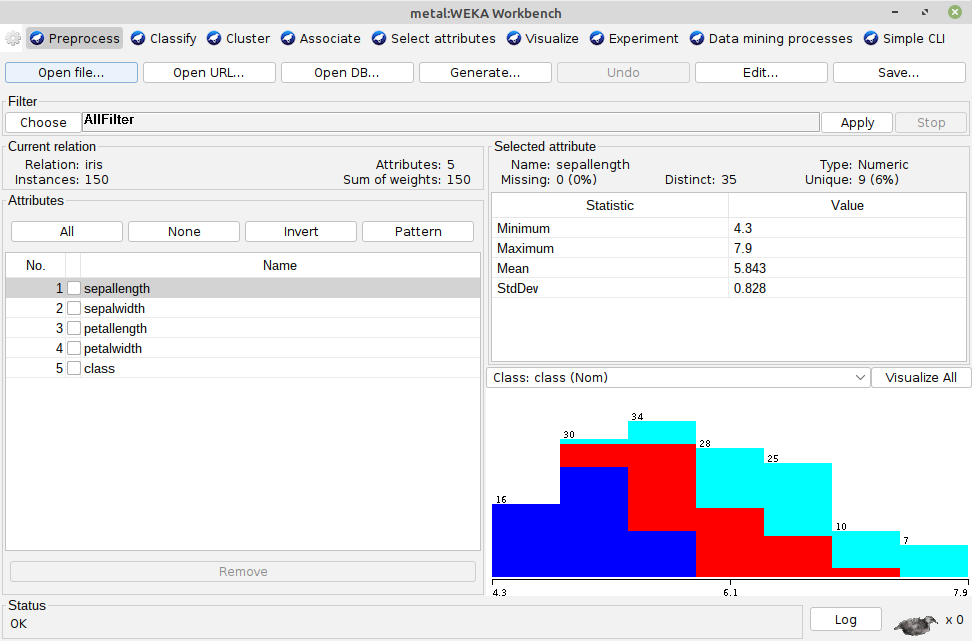
\includegraphics[width=12.0cm]{images/workbench.png}
  \caption{The Workbench interface.}
  \label{workbench}
\end{figure}


% This work is made available under the terms of the
% Creative Commons Attribution-ShareAlike 4.0 license,
% http://creativecommons.org/licenses/by-sa/4.0/.

\chapter{Tools}

\section{WEKA Append datasets}

If you have datasets with the same structure, i.e., exactly the same
attributes, then you can use the \textit{Append datasets} tool to combine
them into a single, large dataset.

The screenshot in Figure \ref{dataset-compatibility} shows the wizard
interface that guides you through the process.

\begin{figure}[htb]
  \centering
  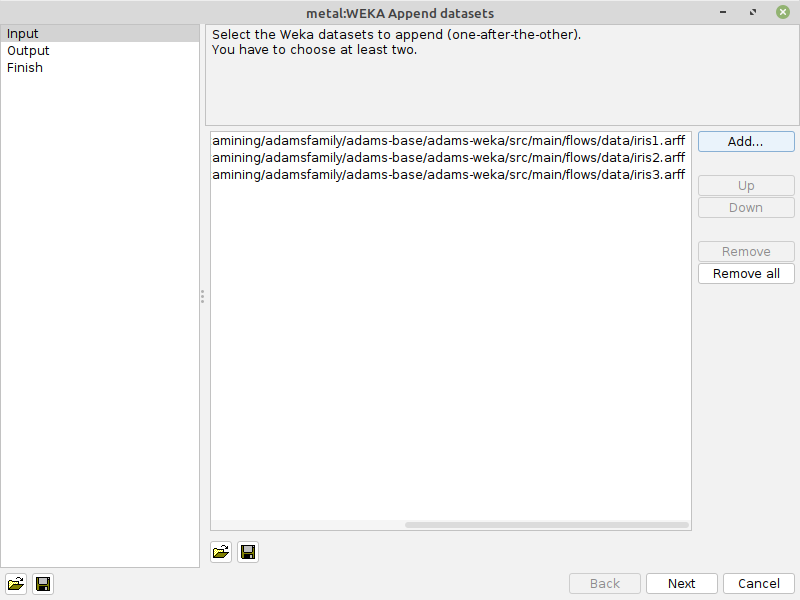
\includegraphics[width=12.0cm]{images/append_datasets.png}
  \caption{Appending datasets wizard.}
  \label{append_datasets}
\end{figure}

\clearpage
\section{WEKA Batch-filter datasets}

Training and test set are required to have exactly the same structure
in WEKA. If you need to apply a pre-processing filter to both of the
files, it is recommended to use \textit{batch-filtering}. This will
ensure that any statistics that get calculated based on the first
dataset, get applied to second file as well. An example for this is
the dictionary of the \textit{StringToWordVector}: the same word
dictionary needs to be applied to the second file, in order to generate
the same attributes. However, one usually has to resort to the command-line
in order to achieve this, which is rather tedious.

The \textit{Batch-filter datasets} wizard allows you to perform the
batch-filtering conveniently through the GUI:
\begin{tight_itemize}
  \item Select the datasets to filter (see \ref{batchfilter_datasets1})
  \item Configure the filter (see \ref{batchfilter_datasets2})
  \item Select the output directory (see \ref{batchfilter_datasets3})
  \item Info dialog after filtering (see \ref{batchfilter_datasets4})
\end{tight_itemize}

\begin{figure}[htb]
  \centering
  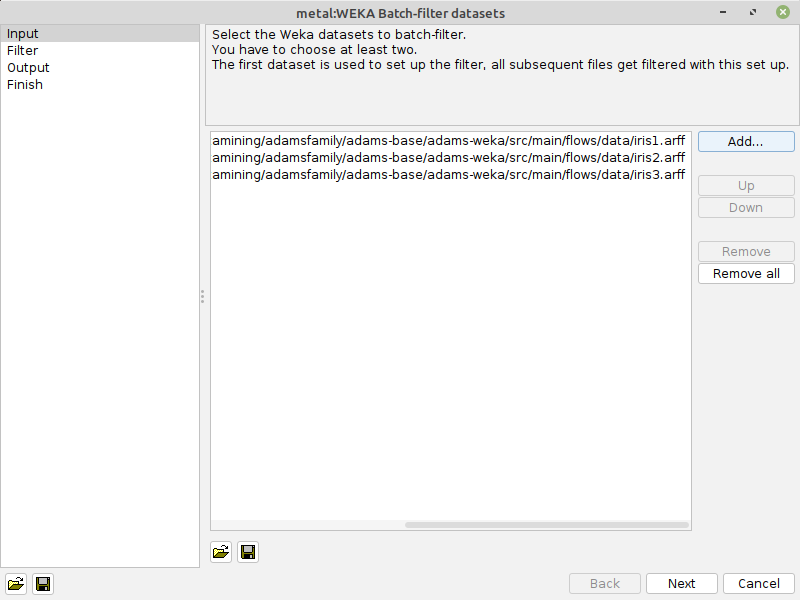
\includegraphics[width=12.0cm]{images/batchfilter_datasets1.png}
  \caption{Selecting input files for batch-filtering.}
  \label{batchfilter_datasets1}
\end{figure}

\begin{figure}[htb]
  \centering
  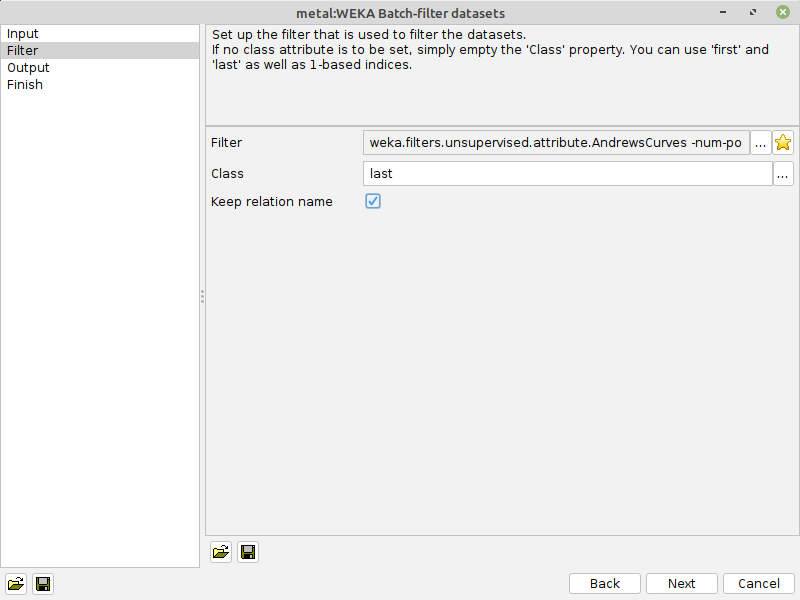
\includegraphics[width=12.0cm]{images/batchfilter_datasets2.png}
  \caption{Configuring the filter.}
  \label{batchfilter_datasets2}
\end{figure}

\begin{figure}[htb]
  \centering
  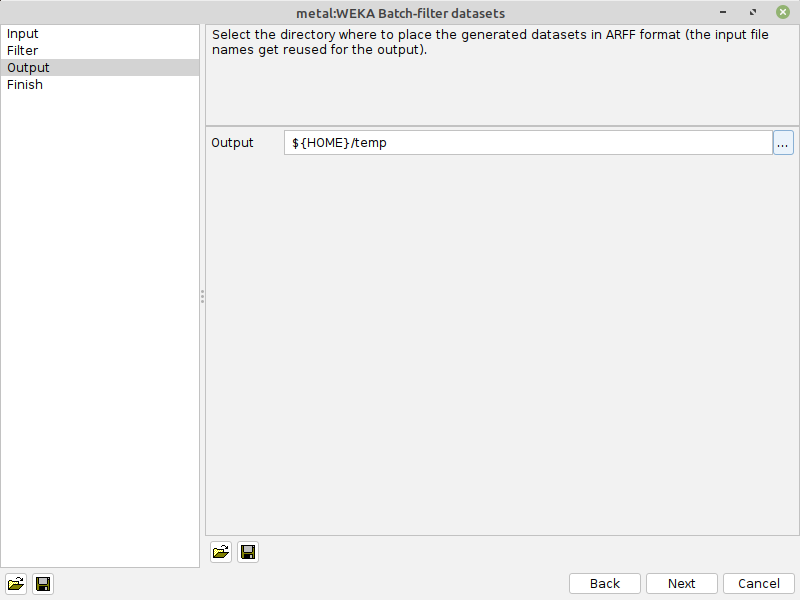
\includegraphics[width=12.0cm]{images/batchfilter_datasets3.png}
  \caption{Selecting the output directory for the filtered datasets.}
  \label{batchfilter_datasets3}
\end{figure}

\begin{figure}[htb]
  \centering
  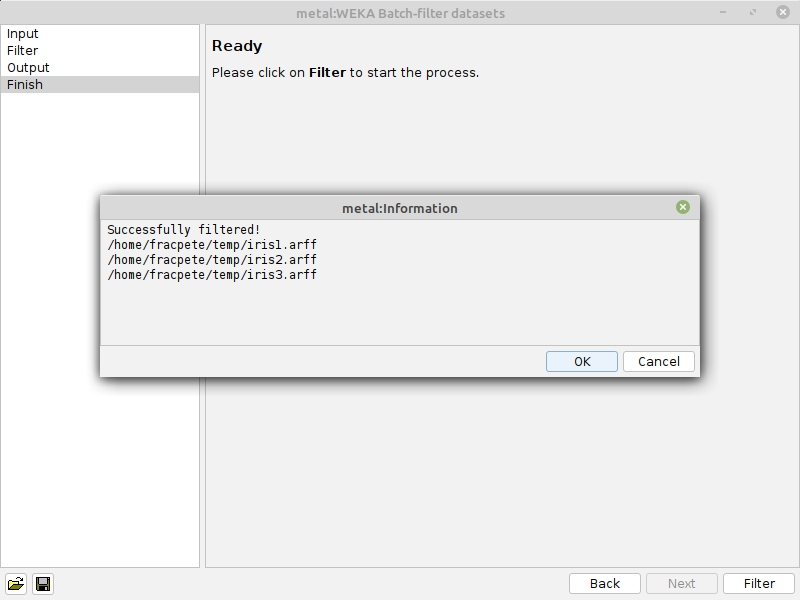
\includegraphics[width=12.0cm]{images/batchfilter_datasets4.png}
  \caption{The dialog when batch-filtering was successful.}
  \label{batchfilter_datasets4}
\end{figure}

\clearpage
\section{WEKA Dataset compatibility}

WEKA requires training and test sets to have the same structure, down to the
same name and order of nominal labels. Rather than relying on the error message
in the Explorer, you can use the \textit{Dataset compatibility} tool to 
quickly check whether two or more datasets are actually compatible.

The screenshot in Figure \ref{dataset-compatibility} shows the output when
comparing two datases, one being the original \textit{anneal} UCI dataset
and the other one a transformed version.

\begin{figure}[htb]
  \centering
  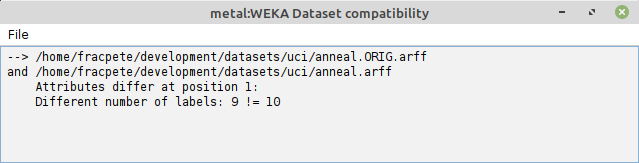
\includegraphics[width=12.0cm]{images/dataset-compatibility.png}
  \caption{Compatibility output for two datasets.}
  \label{dataset-compatibility}
\end{figure}

\clearpage
\section{WEKA Make compatible datasets}
When dealing with data across multiple spreadsheets, e.g., training, test
and validation set, then it can happen that these datasets are not compatible
in the strict Weka sense.

The \textit{Make compatible datasets} wizard allows you to turn spreadsheets
into compatible ARFF files:
\begin{tight_itemize}
  \item Select the datasets to make compatible (see \ref{makecompatible1})
  \item Configure how the datasets are being read (see \ref{merge_datasets2})
  \item Select the output directory for the compatible ARFF files (see \ref{merge_datasets3})
  \item Info dialog after processing the datasets (see \ref{merge_datasets4})
\end{tight_itemize}

\begin{figure}[htb]
  \centering
  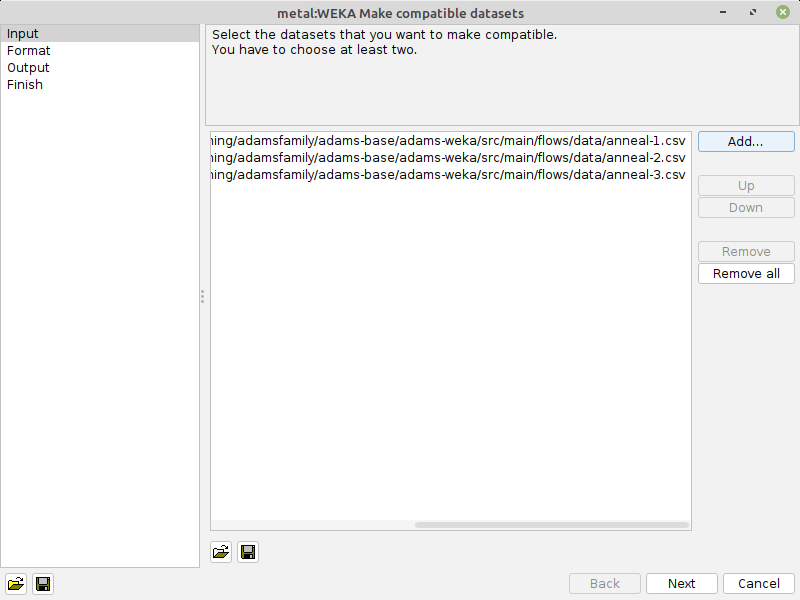
\includegraphics[width=12.0cm]{images/makecompatible1.png}
  \caption{Selecting input files for making compatible datasets.}
  \label{makecompatible1}
\end{figure}

\begin{figure}[htb]
  \centering
  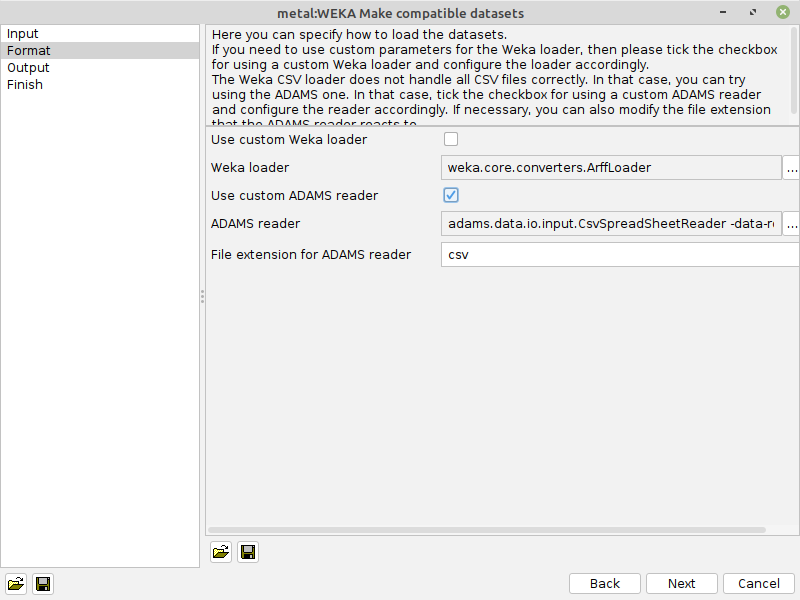
\includegraphics[width=12.0cm]{images/makecompatible2.png}
  \caption{Configuring the readers for the datasets.}
  \label{makecompatible2}
\end{figure}

\begin{figure}[htb]
  \centering
  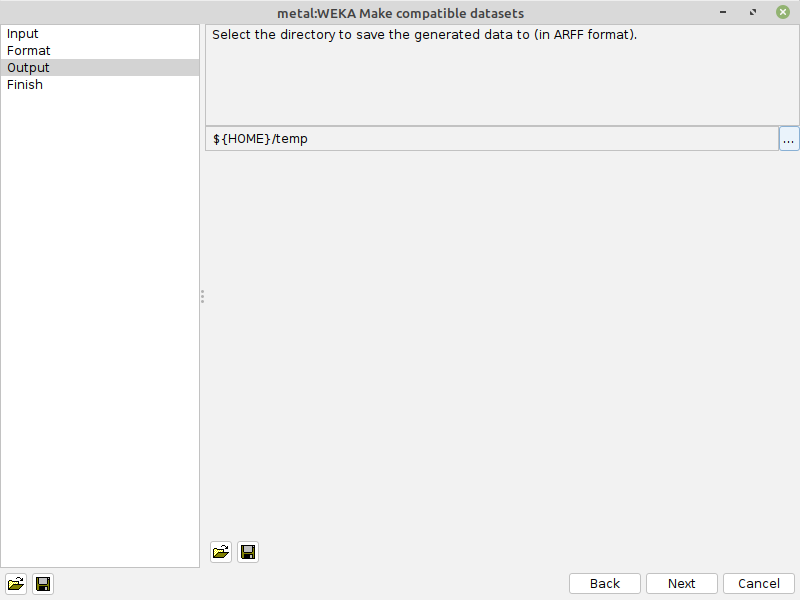
\includegraphics[width=12.0cm]{images/makecompatible3.png}
  \caption{Selecting the output directory for the compatible ARFF files.}
  \label{makecompatible3}
\end{figure}

\begin{figure}[htb]
  \centering
  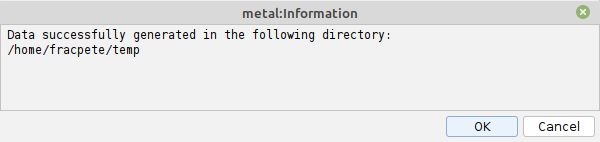
\includegraphics[width=8.0cm]{images/makecompatible4.png}
  \caption{The dialog when dataset generation was successful.}
  \label{makecompatible4}
\end{figure}

\clearpage
\section{WEKA Merge datasets}
The process of adding reference data to a dataset or performing
\textit{data fusion}\footnote{\url{https://en.wikipedia.org/wiki/Data_fusion}{}},
can be quite often a manual process, copy/pasting datasets in a spreadsheet
application.

The \textit{Merge datasets} wizard allows you to perform the
process of combining datasets side-by-side conveniently in the GUI:
\begin{tight_itemize}
  \item Select the datasets to merge (see \ref{merge_datasets1})
  \item Configure the merge (see \ref{merge_datasets2})
  \item Select the output file (see \ref{merge_datasets3})
  \item Info dialog after merging (see \ref{merge_datasets4})
\end{tight_itemize}
Figure \ref{merge_datasets-output} shows an example of a merged file.

\begin{figure}[htb]
  \centering
  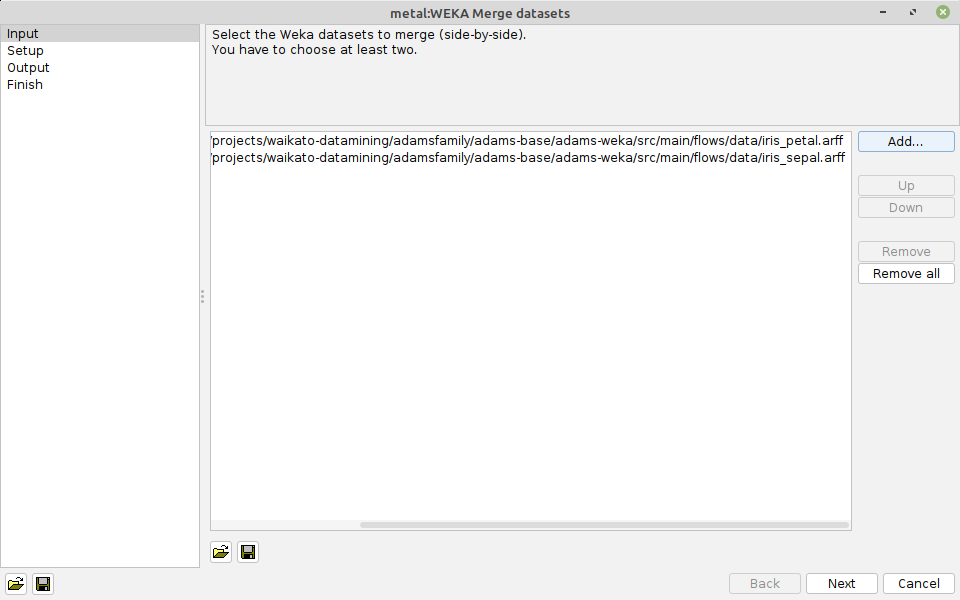
\includegraphics[width=12.0cm]{images/merge_datasets1.png}
  \caption{Selecting input files for merging.}
  \label{merge_datasets1}
\end{figure}

\begin{figure}[htb]
  \centering
  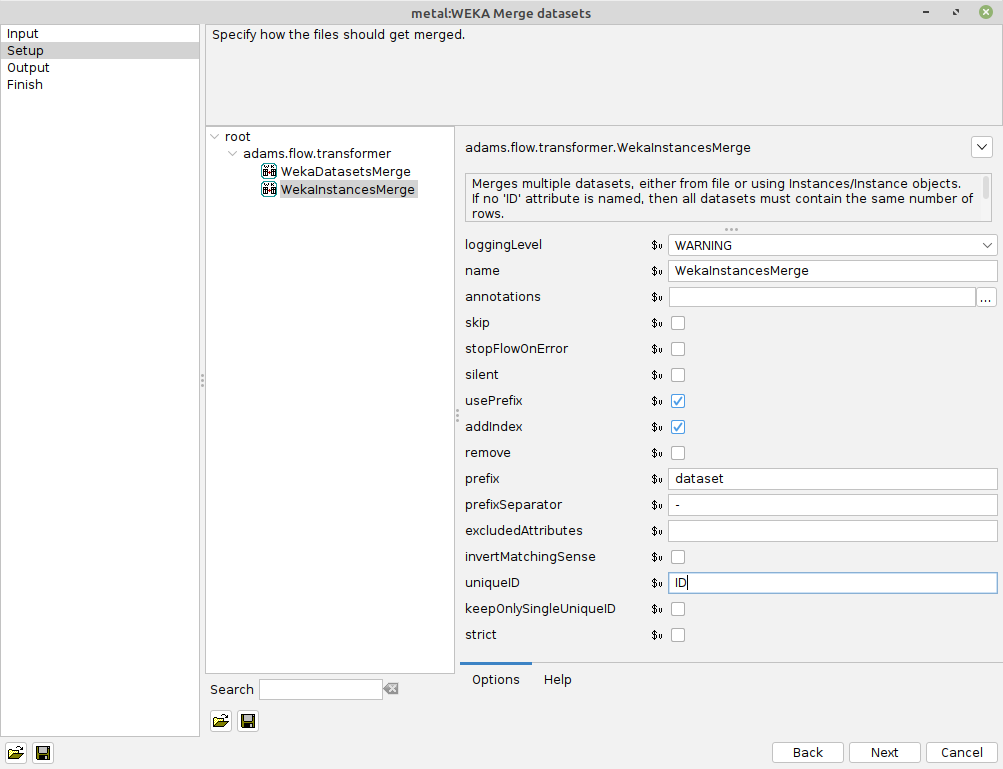
\includegraphics[width=12.0cm]{images/merge_datasets2.png}
  \caption{Configuring the merge.}
  \label{merge_datasets2}
\end{figure}

\begin{figure}[htb]
  \centering
  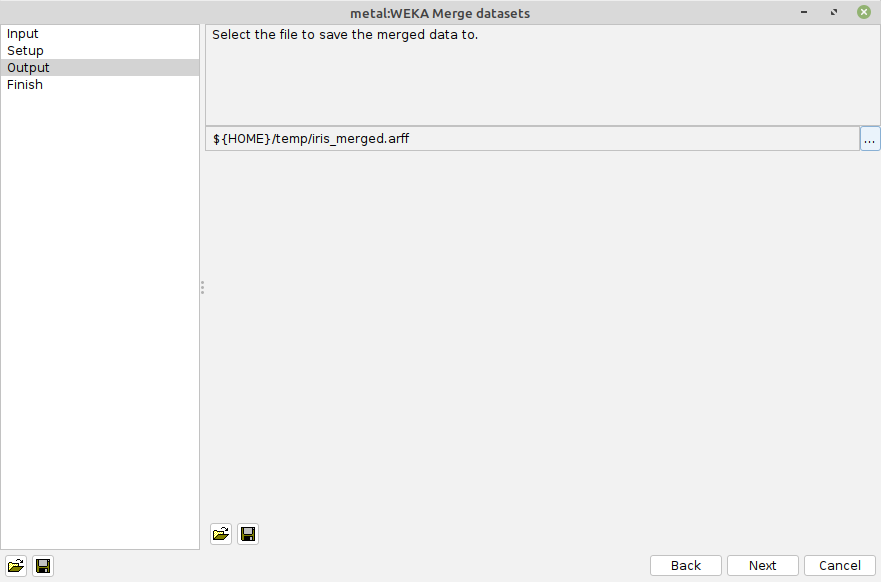
\includegraphics[width=12.0cm]{images/merge_datasets3.png}
  \caption{Selecting the file to save the merged dataset to.}
  \label{merge_datasets3}
\end{figure}

\begin{figure}[htb]
  \centering
  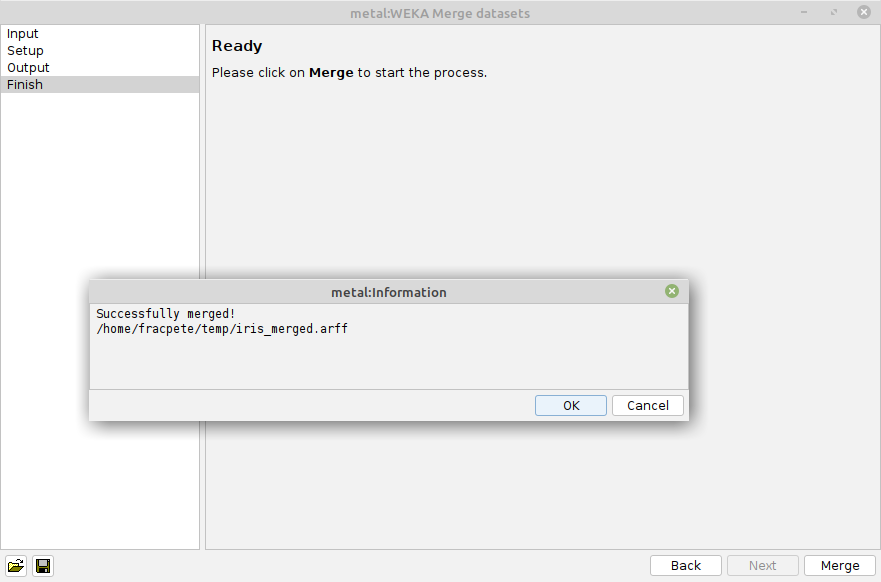
\includegraphics[width=12.0cm]{images/merge_datasets4.png}
  \caption{The dialog when merging was successful.}
  \label{merge_datasets4}
\end{figure}

\begin{figure}[htb]
  \centering
  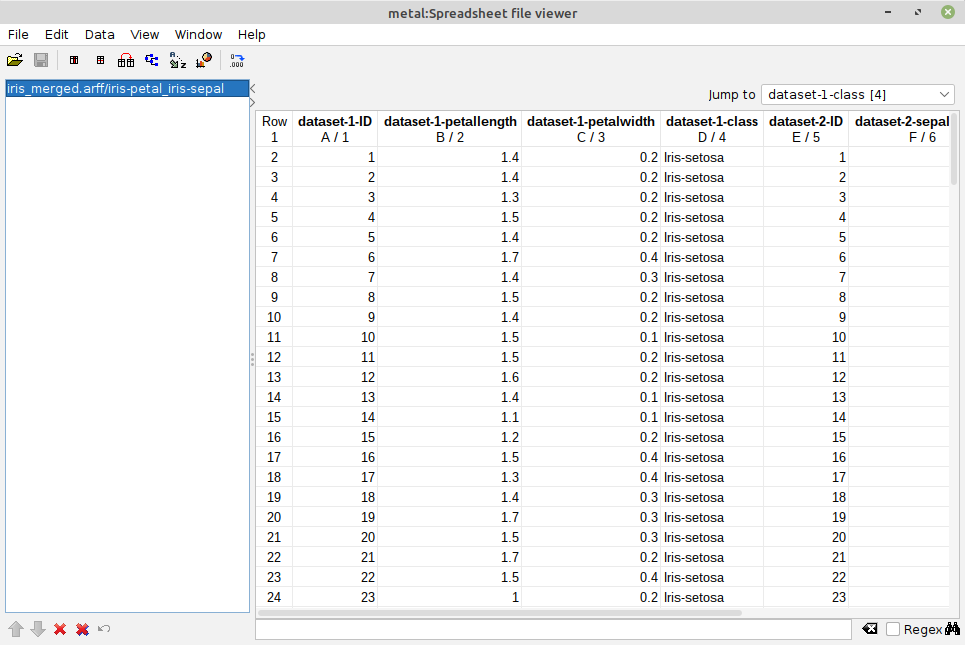
\includegraphics[width=12.0cm]{images/merge_datasets-output.png}
  \caption{The merged dataset.}
  \label{merge_datasets-output}
\end{figure}


\chapter{Logging}
Weka performs its own logging of stdout and stderr, which can amount to very
large log files on the server, which will never get cleared. In order to
turn off logging, perform the following steps:
\begin{tight_itemize}
  \item create the following directory if not already present: \verb|$HOME/wekafiles/props|
  (or \verb|%USERPROFILE%\wekafiles\props| for Windows)
  \item in this directory, create file \textit{Logging.props} with the following content:
  \begin{verbatim}
weka.core.logging.Logger=weka.core.logging.ConsoleLogger
  \end{verbatim}
\end{tight_itemize}

%%%%%%%%%%%%%%%%%%%%%%%%%%%%%%%%%%%
% This work is made available under the terms of the 
% Creative Commons Attribution-ShareAlike 4.0 license,
% http://creativecommons.org/licenses/by-sa/4.0/.

\begin{thebibliography}{999}
	% to make the bibliography appear in the TOC
	\addcontentsline{toc}{chapter}{Bibliography}

    % references
	\bibitem{adams}
		\textit{ADAMS} -- Advanced Data mining and Machine learning System \\
		\url{https://adams.cms.waikato.ac.nz/}{}

	\bibitem{jep}
	 	\textit{Jep} -- Java Embedded Python \\
		\url{https://github.com/ninia/jep}{}

	\bibitem{weka}
	 	Mark Hall, Eibe Frank, Geoffrey Holmes, Bernhard Pfahringer, Peter
	 	Reutemann, Ian H. Witten (2009); \textit{The WEKA Data Mining Software: An
	 	Update}; SIGKDD Explorations, Volume 11, Issue 1. \\
		\url{https://ml.cms.waikato.ac.nz/weka/}{}

\end{thebibliography}


\end{document}
